\documentclass[../main.tex]{subfiles}

\begin{document}
\section{Linear models for classification}
The goal in classification is to take an
input vector x and to assign it to one of K discrete classes $C_k$ where $k = 1,...,K$.
In the most common scenario, the classes are taken to be disjoint, so that each input is
assigned to one and only one class. The input space is thereby divided into decision
regions whose boundaries are called decision boundaries or decision surfaces. In
this chapter, we consider linear models for classification, by which we mean that the
decision surfaces are defined by (D - 1)-dimensional hyperplanes within the D-dimensional input space. Data
sets whose classes can be separated exactly by linear decision surfaces are said to be
linearly separable.

\subsection{Linear classification}
We will consider linear models for classification. In the linear regression case, the model is linear in parameters,
\begin{align*}
    y(x,w) & = \sum_{j=0}^{D-1} w_jx_j = x^Tw                                                  \\
           & \text{To have a simpler notation in future steps we explicit }w_0 \text{ from } w \\
           & = w_0 + \sum_{j=1}^{D-1} w_jx_j = w_0 + x^Tw \numberthis
\end{align*}
For classification, we need to predict discrete class labels, or posterior probabilities that lie in the range of $(0,1)$, so we use a nonlinear function(discriminant function) to remap the input space to the output space.
\begin{equation*}
    y(x,w) = \underbrace{f(w_0 + x^Tw)}_{\text{activation function}}
\end{equation*}
A naive way to perform classification with two output classes is to choose an arbitrary activation function and for output less than $0.5$ we have class 0 and viceversa class 1. We could be tricked into thinking that this classifier can predict nonlinear boundaries, but it's not the case. In fact, taken the boundary
\begin{align*}
    f(w_0 + x^Tw)           & = 0.5                                   \\
    f^{-1}(f(w_0 + x^Tw))   & = f^{-1}(0.5)                           \\
    w_0 + x^Tw              & = f^{-1}(0.5)                           \\
    w_0^* + x^Tw            & = 0, \numberthis \label{eqn_hyperplane} \\
    \text{with} \quad w_0^* & = w_0 - f^{-1}(0.5)
\end{align*}
As we can see (\ref{eqn_hyperplane}) represents an hyperplane, hence the decision surfaces are linear functions of x, even if the activation function is nonlinear. As in regression we can use basis function to make the input space linearly separable. The bad thing about this approach is that the model is no longer linear in the parameters, so no closed form solution exists.
\subsubsection{Geometric interpretation}
To have a better understanding of the discriminant function we can analyze it from a geometric point of view. The simplest representation of a linear discriminant function is obtained by taking a linear function of the input vector so that $y(x,w) = w_0 + x^Tw$. $w_0$ is called bias and its negative is called threshold. An input vector x is assigned to class $C_1$ if $y(x) \geq 0$ and to class $C_2$ otherwise. The corresponding decision boundary is therefore defined by the relation $y(x)=0$, which corresponds to a (D - 1)-dimensional hyperplane within the D-dimensional input space. Consider two points $x_A$ and $x_B$ both of which lie on the decision surface.
Because $y(x_A) = y(x_B)=0$, we have $w^T(x_A -x_B)=0$ and hence the vector w is orthogonal to every vector lying within the decision surface\footnotemark, and so w determines the
orientation of the decision surface.
\footnotetext{Given two vector their dot product is 0 when they are perpendicular to each other. $a \cdot b = |a||b|cos\theta$}
We can also say that $w_0$ regulates the normal distance(d) of the boundary from the origin. To find r we can project\footnotemark a point x on the boundary on w
\begin{align*}
    w^Tx + w_0               & = 0                                \\
    w^Tx                     & = -w_o                             \\
    d = \frac{w^Tx}{\|w\|_2} & = -\frac{w_0}{\|w\|_2} \numberthis
\end{align*}
\footnotetext{We know that the projection of a vector a on another vector b is $proj_b(a) = \frac{ab}{\|b\|}$.}
\begin{center}
    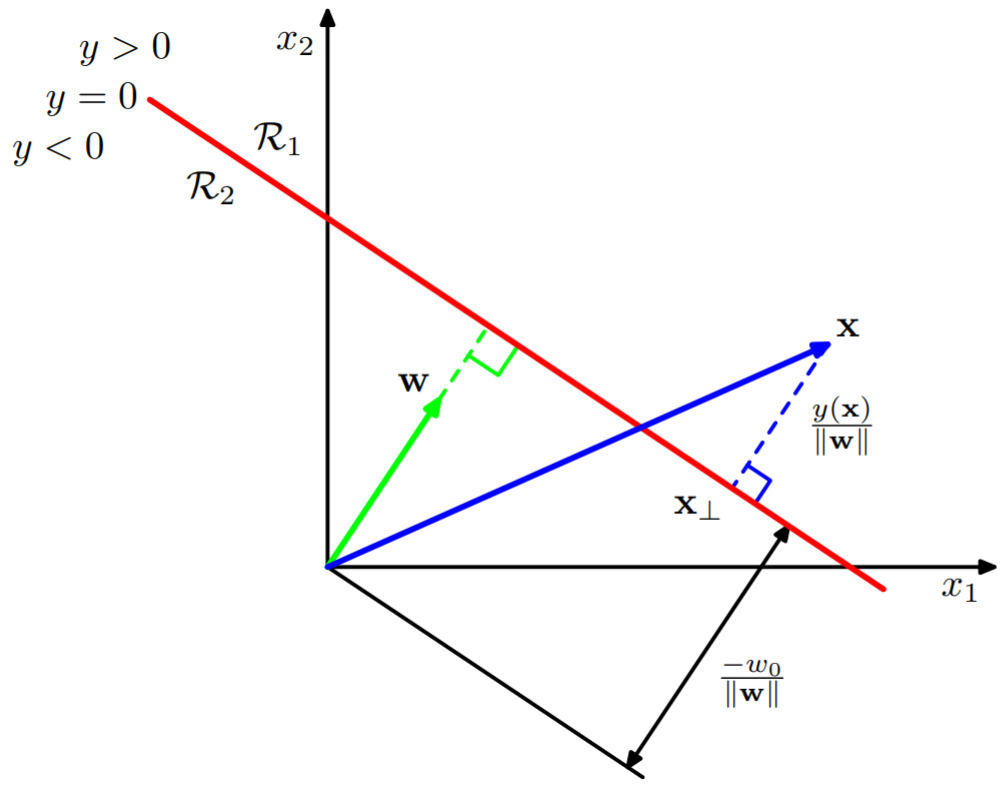
\includegraphics[scale=0.6]{images/Linearboundary.PNG}
\end{center}
Furthermore, we can obtain the signed distance(r) of a point x from the boundary. Let's consider the projection $x_{\perp}$ of x on the boundary. Then
\begin{align*}
    x          & = x_{\perp} + r\frac{w}{\| w \|_2}                                 \\
    w^Tx       & = w^T x_{\perp} + w^T r\frac{w}{\| w \|_2}                         \\
    w^Tx + w_0 & = \underbrace{w^T x_{\perp} + w_0}_{=0} + w^T r\frac{w}{\| w \|_2} \\
    y(x)       & = w^T r\frac{w}{\| w \|_2}                                         \\
    y(x)       & = r\frac{\| w \|_2^2}{\| w \|_2}                                   \\
    r          & = \frac{y(x)}{\| w \|_2} \numberthis
\end{align*}

\subsubsection{Multiple outputs}
Now consider the extension of linear discriminants to $K>2$ classes. We might be tempted be to build a K-class discriminant by combining a number of two-class discriminant functions. However, this leads to some serious difficulties.
\paragraph{One-versus-the-rest}
Consider the use of K-1 classifiers each of which solves a two-class problem of separating points in a particular class $C_k$ from points not in that class. There are regions in input space that are ambiguously classified, as we can see in the left-hand diagram.
\paragraph{One-versus-one}
An alternative is to introduce K(K - 1)/2 binary discriminant functions, one for every possible pair of classes. Each
point is then classified according to a majority vote amongst the discriminant functions. However, this too runs into the problem of ambiguous regions, as illustrated in the right-hand diagram.
\begin{center}
    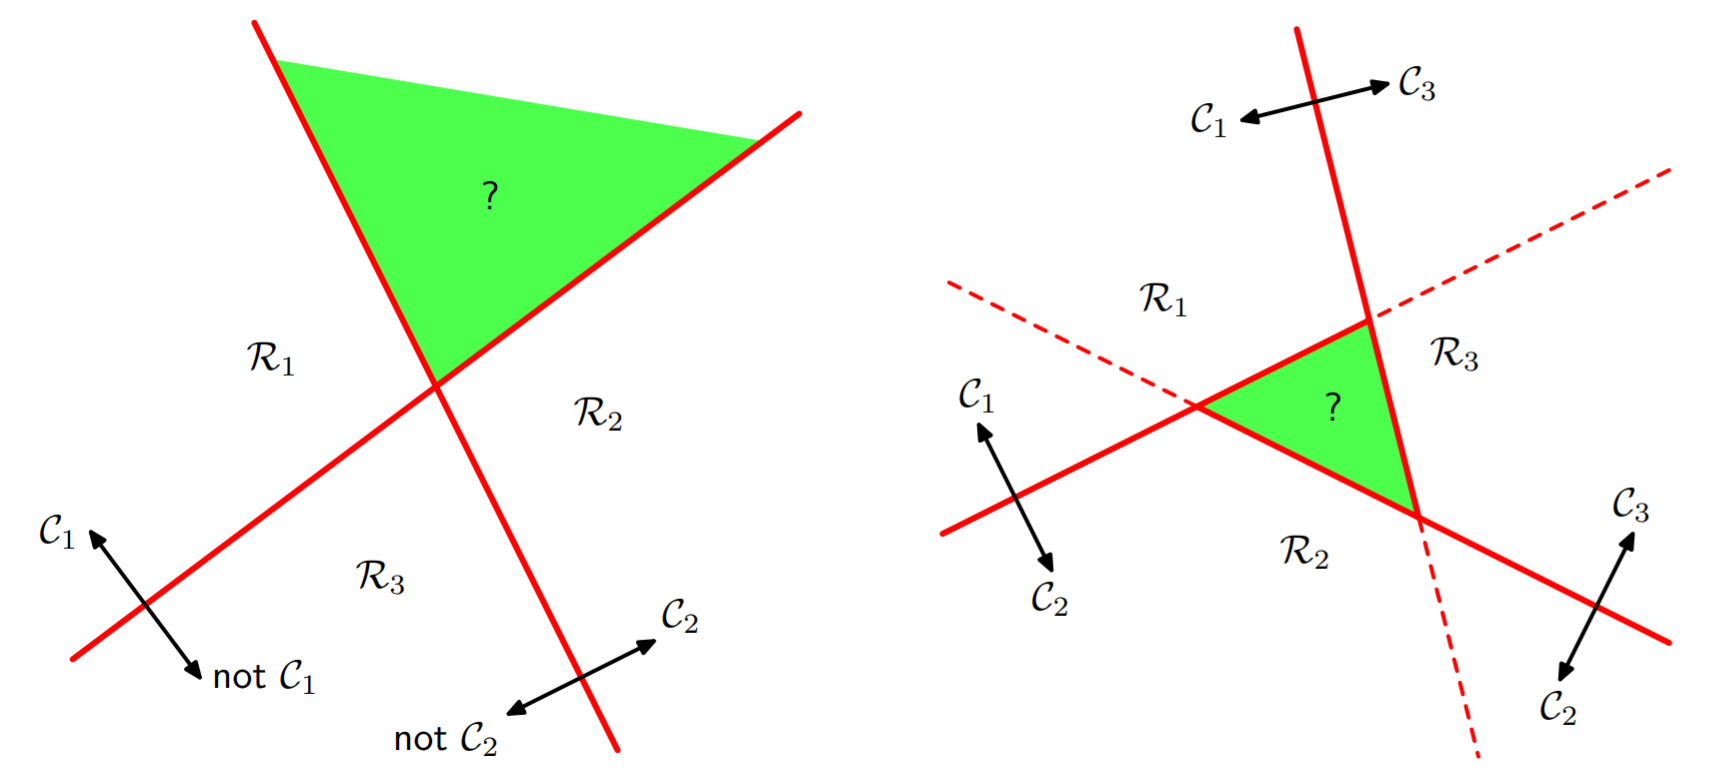
\includegraphics[scale=0.5]{images/Multiclass_classification.PNG}
\end{center}

\newpage
\paragraph{Linear discriminant functions}
We can avoid these difficulties by considering a single K-class discriminant comprising K linear functions of the form
\begin{equation}
    y_k(x) = w_k^Tx + w_{ko},\quad where \quad k=1,\dots,K
\end{equation}
and then assigning a point x to class $C_k$ if $y_k(x) > y_j (x), \quad \forall j \neq k$. The decision boundary between class $C_k$ and class $C_j$ is therefore given by $y_k(x) = y_j(x)$ and hence corresponds to a (D - 1)-dimensional hyperplane.
The resulting decision boundaries are singly connected\footnotemark and convex. \footnotetext{It means that all the linear functions are ray originating from a common point}Convexity imposes that taken two points $x_A$ and $x_B$ that belong to the same region $R_k$, every point $\hat{x}$ in between is still inside region $R_k$
\begin{equation*}
    \hat{x} = \lambda x_A + (1-\lambda)x_B, \quad \hat{x}\in R_k. \quad \lambda \in [0, 1]
\end{equation*}
Convexity and linearity of the discriminant functions imply that
\begin{equation*}
    f_k(\lambda x_A + (1-\lambda)x_B) > f_j(\lambda x_A + (1-\lambda)x_B), \quad \forall j \in [1, K] \setminus k
\end{equation*}

\subsection{Least square for classification}
Consider a general classification problem with K classes, with a one-hot encoding for the target vector t. One justification for using least squares in such a context is that it approximates the conditional expectation $E[t|x]$ of the target values given the input vector.
Each class is described by its own linear model
\begin{equation}
    y_k(x) = w_k^Tx + w_{ko},\quad where \quad k=1,\dots,K
\end{equation}
Using vector notation,
\begin{gather*}
    y(x) = \Tilde{W}^T \Tilde{x}, \quad where \\
    \Tilde{W}=
    \begin{bmatrix}
        \begin{bmatrix}
            w_{10} \\ \vdots \\ w_{1D}
        \end{bmatrix}_{w_1^T}
         & \dots &
        \begin{bmatrix}
            w_{K0} \\ \vdots \\ w_{KD}
        \end{bmatrix}_{w_K^T}
    \end{bmatrix},\quad [D+1 x K] \\
    \Tilde{x}=(1, x^T)^T, \quad [D+1 x 1]
\end{gather*}
We classify the input x into class $C_k$ if $y_k(x)>y_j(x), \quad \forall j \in [1, K] \setminus k$. $y_k(x)$ corresponds to the $k^{th}$ element of $y(x)$.
To estimate the parameter we can follow what we did for the regression problem. To minimize least square,
\begin{gather*}
    \Tilde{W} = (\Tilde{X}^T \Tilde{X})^{-1} \Tilde{X}^T T, \quad [(D+1) x K] \numberthis \\
    \Tilde{X} \quad [N x (D+1)] \\
    \Tilde{T} \quad [N x K]
\end{gather*}
\subsubsection{Least squares problems}
The least square approach is problematic in some cases.
\paragraph{Outliers} Least square is very sensitive to outliers. Least square tries to find a line which is the most close to all points. It does so evaluating the square distance between the samples and the line. It means that an outlier will have a greater impact on the line position because it will be more distant with respect to the probable samples. In classification this could degrade a lot the performance, because the boundary could deviate so much that some samples, previously well classified, now lie on the other side of the boundary.
\begin{center}
    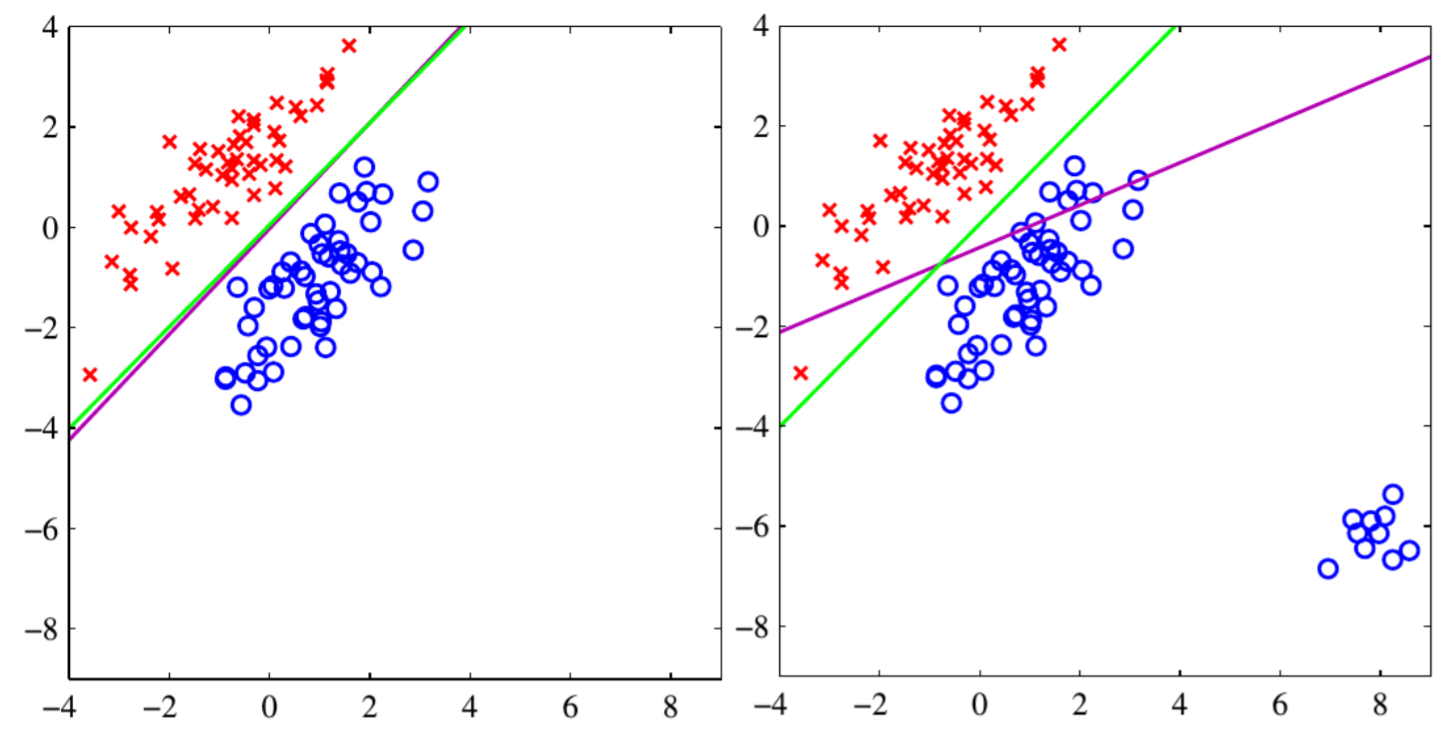
\includegraphics[scale=0.50]{images/LS_Outliers.PNG}
\end{center}

\paragraph{Non-Gaussian distributions}
We recall that least squares corresponds to the maximum likelihood under the assumption of a Gaussian conditional distribution, whereas binary target vectors clearly have a distribution that is far from Gaussian. As we can see in the figure below, even though the three classes are linearly separable, least square is not able to find good boundaries.
\begin{center}
    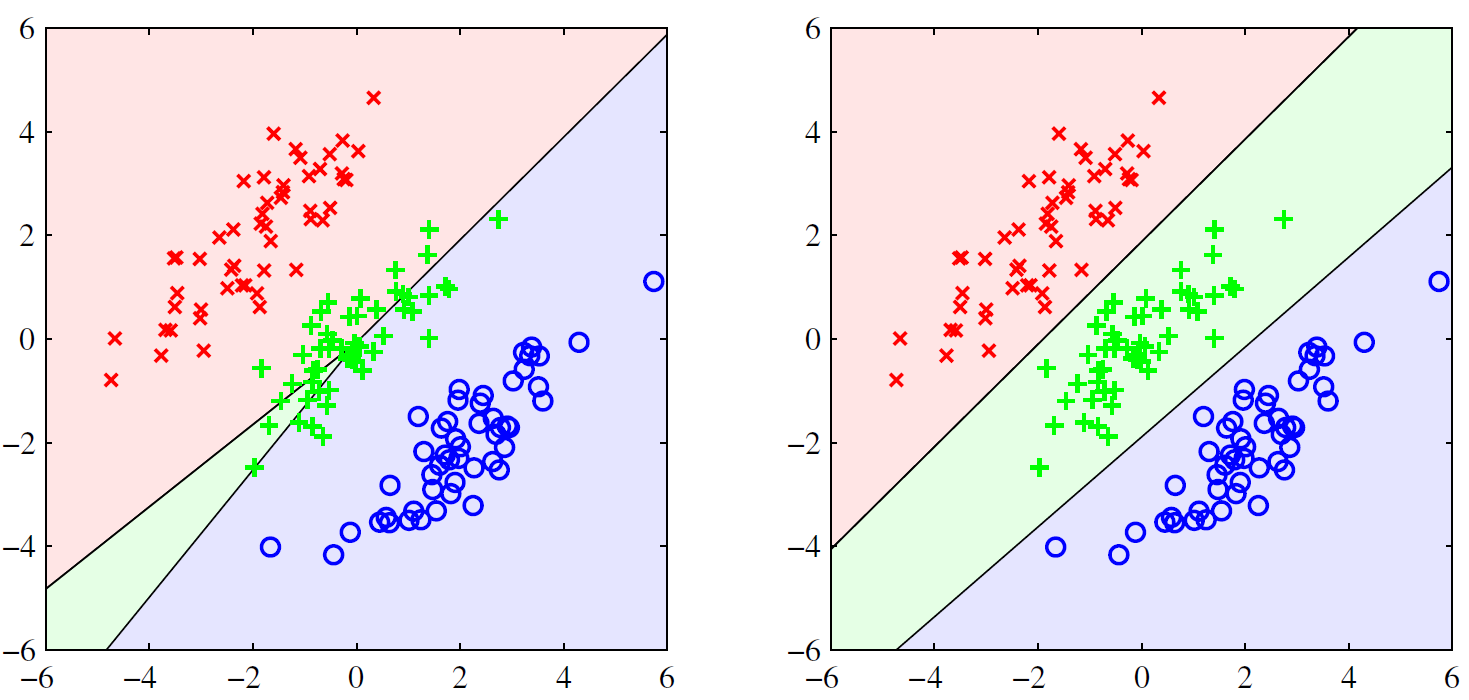
\includegraphics[scale=0.40]{images/LS_nongaussian.PNG}
\end{center}

\newpage
\subsubsection{Basis functions}
So far, we have considered classification models that work directly in the input space. All considered algorithms are equally applicable if we first make a fixed nonlinear transformation of the input space using vector of basis functions $\Phi(x)$. Decision boundaries will be linear in the feature space, but would correspond to nonlinear boundaries in the original input space.
\paragraph{Example - Nonlinear basis}
Illustration of the role of nonlinear basis functions in linear classification models. The left plot shows the original input space $(x_1, x_2)$ together with data points from two classes labelled red and blue. Two
‘Gaussian’ basis functions $\Phi_1(x)$ and $\Phi_2(x)$ are defined in this space with centres shown by the green crosses
and with contours shown by the green circles. The right-hand plot shows the corresponding feature space $(\Phi_1(x), \Phi_2(x))$ together with the linear decision boundary. This corresponds to a nonlinear decision boundary in the original input space, shown by the black curve in the left-hand plot.
\begin{center}
    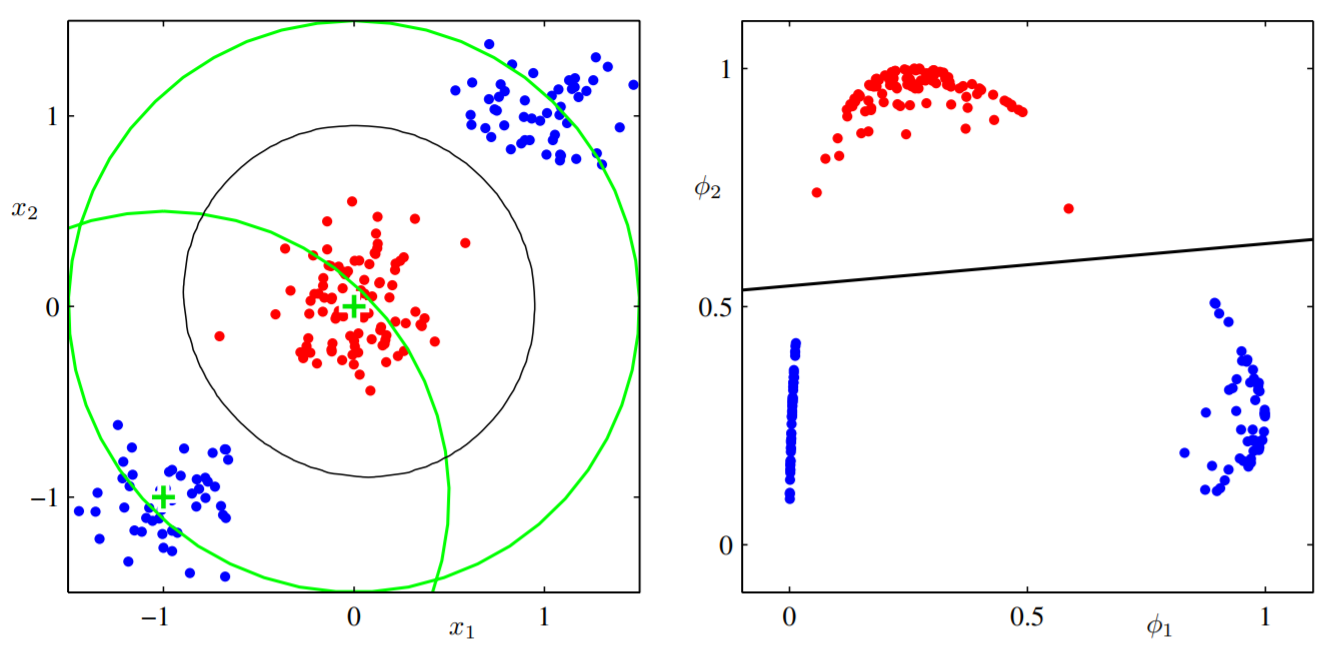
\includegraphics[scale=0.50]{images/LS_Gaussian_Basis.PNG}
\end{center}

\subsection{Perceptron}
The perceptron is an algorithm for online\footnotemark supervised learning of binary classifiers. \footnotetext{Online means that it is an iterative approach which calculate the solutions with multiple steps}The algorithm tries to find a threshold function: a function that maps its input x (a real-valued vector) to an output value
\begin{align*}
    y(x)= f(w^T\Phi(x)), \quad where \\
    f(a) =
    \begin{cases}
        +1, & a \geq 0 \\
        -1, & a < 0
    \end{cases}
\end{align*}
Target values are +1 for $C_1$ and -1 for $C_2$. The algorithm finds the separating hyperplane by minimizing the distance of misclassified points to the decision boundary.
Our objective is to find a parameter vector $w$ such that $w^T \Phi(x_n) \geq 0$ when $x_n \in C_1$ and $w^T \Phi(x_n) < 0$ when $x_n \in C_2$.
Now we define an error function as follow,
\begin{align*}
    \epsilon_p(w, x_n) =
    \begin{cases}
        0,               & \text{If x is classified correctly}                                         \\
        w^T\Phi(x_n)t_n, & \text{If x is not classified correctly (proportional to boundary distance)}
    \end{cases}
\end{align*}
Now we define an error function for the parameter optimization,
\begin{equation}
    L_P(w) = -\sum_{n \in M}w^T\Phi(x_n)t_n
\end{equation}
To perform minimization we use stochastic gradient descent(online)
\begin{equation}
    w^{(k+1)} = w^{(k)} - \alpha \nabla L_P(w) = w^{(k)} + \alpha \Phi(x_n)t_n
\end{equation}

\paragraph{Note - Loss sign} We have a minus sign in the loss function because $w^T\Phi(x_n)t_n$ will always be negative. This is due to the fact that if $w^T\Phi(x_n)$ is misclassified, then it will have an opposite sign compared to $t_n$.
\paragraph{Note - Learning rate} The learning rate $\alpha$ can be set to 1 because it doesn't change the direction of w. We assume that w starts from the origin, so a scaling of the vector doesn't affect the boundary definition.

\subsubsection{Perceptron algorithm}
\begin{algorithm}[H]
    \SetAlgoLined
    \SetKwInOut{Input}{Input}
    \SetKwInOut{Output}{Output}
    \SetKwInOut{Initialize}{Initialize}
    \Output{A parameter vector $w^{(k)}$ that correctly classifies the two classes}
    \Input{Data set $x_n \in \mathbb{R}^D$ \newline
        $t_n \in \{-1,+1\}$, $\forall n \in [1,N]$
    }
    \Initialize{$w_0$}
    $k \leftarrow 0$\;
    \While{!converged}{
        $k \leftarrow k+1$\;
        $n \leftarrow k\%N$\;
        \If{$\hat{t_n} \neq t_n$}{
            $w^{(k+1)} \leftarrow w^{(k)} + \Phi(x_n)t_n$\;
        }
    }
    \caption{Perceptron algorithm}
\end{algorithm}

\begin{center}
    \begin{tabular}{cc}
        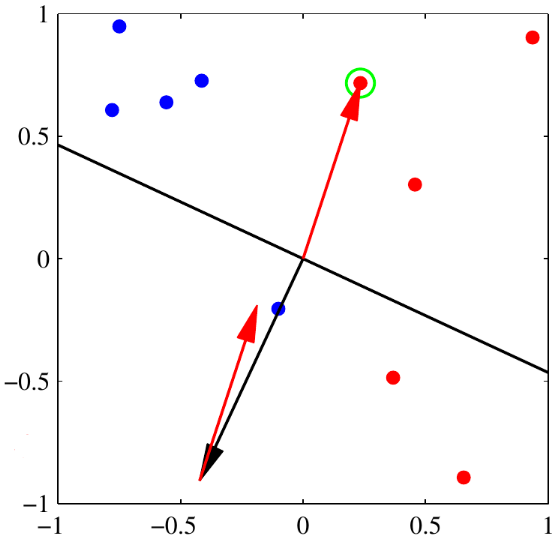
\includegraphics[width=65mm]{images/Perceptron_Alg1.PNG} & 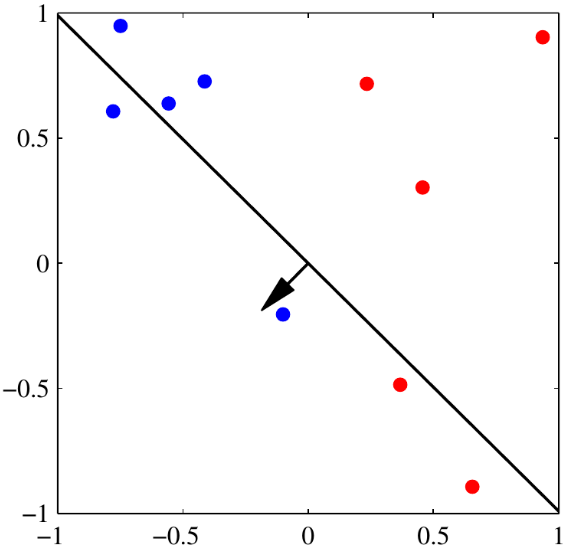
\includegraphics[width=65mm]{images/Perceptron_Alg2.PNG} \\
        (a)                                                      & (b)                                                      \\[6pt]
        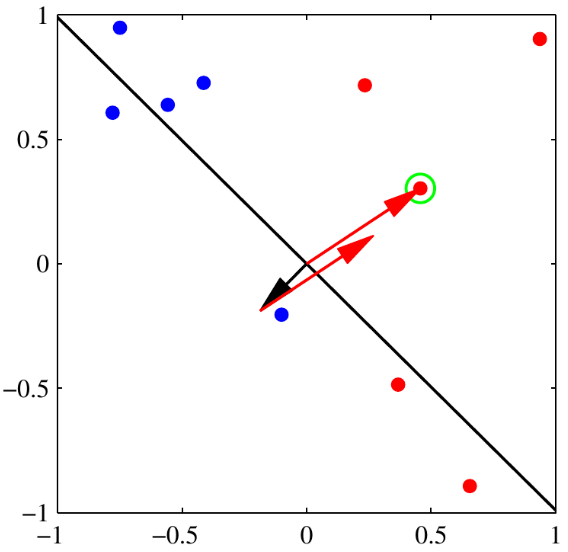
\includegraphics[width=65mm]{images/Perceptron_Alg3.PNG} & 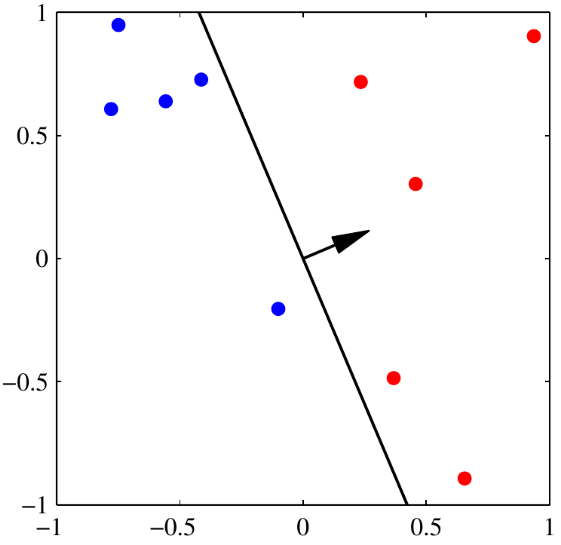
\includegraphics[width=65mm]{images/Perceptron_Alg4.PNG} \\
        (c)                                                      & (d)                                                      \\[6pt]
    \end{tabular}
\end{center}

\begin{theorem}[Perceptron convergence theorem]
    If the training data set is linearly separable in the feature space $\Phi$, then the perceptron learning algorithm is guaranteed to find an exact solution in a finite number of steps
\end{theorem}
The number of steps before convergence may be substantial. We are not able to distinguish between non-separable problems and slowly converging ones. If multiple solutions exist, the one found depends by the initialization of the parameters and the order of presentation of the data points.
Another fact about algorithm steps is that the effect of a single update is to reduce the error due to the misclassified pattern, but this does not imply that the loss is reduced at each stage. This means that we reduce the error of the misclassified point we are considering, but we have no guarantee that the error of the other points gets better.

\newpage
\subsection{Logistic regression}
Logistic regression is a statistical model that in its basic form uses a logistic function to model a binary variable. So it is capable of resolve two-class classification.
Logistic regression is a discriminative model so we model directly the posterior probability $P(C_k|\Phi)$. In detail we use a logistic sigmoid function\footnotemark.
\begin{align}
    P(C_1|\Phi) & = \sigma(w^T \Phi) = \frac{1}{1+e^{-w^T\Phi}} \\
    P(C_2|\Phi) & = 1- P(C_1|\Phi)
\end{align}
\footnotetext{Sigmoid function: $\sigma(x)=\frac{1}{1+e^{-x}}$}

\paragraph{Note} Logistic regression is a classification method not a regression one.

\begin{center}
    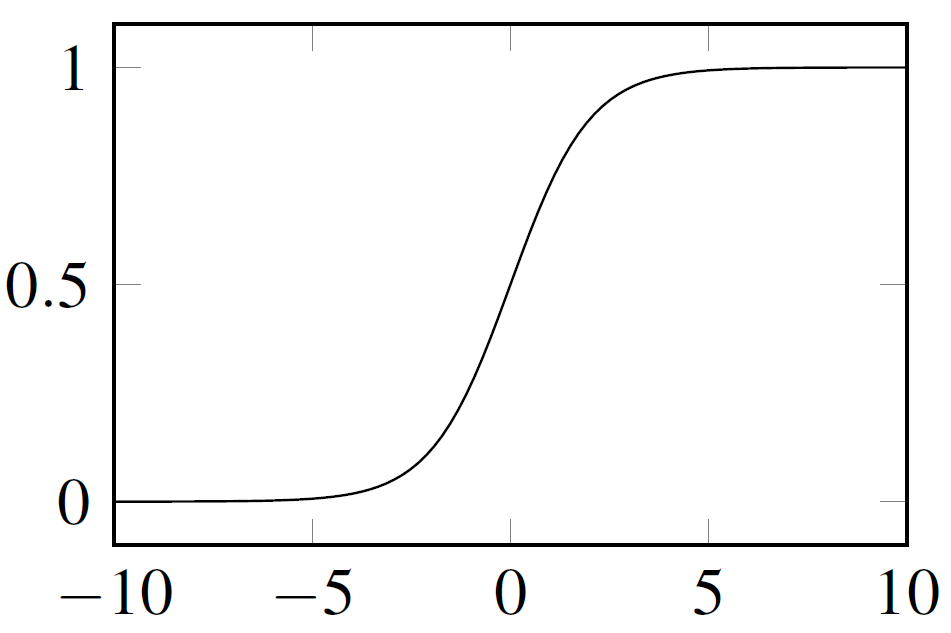
\includegraphics[scale=0.4]{images/Sigmoid.PNG}
\end{center}

\subsubsection{Maximum Likelihood for logistic regression}
We now use maximum likelihood to determine the parameters of the logistic regression model. Now we have to define a suitable loss function to use. To do so, we first analyze our inputs and outputs. We have a dataset $D = \{x_n, t_n\},$ $n=1,\dots,N$
\begin{align*}
    y_n(\Phi(x_n)|w) = P(t_n|\Phi(x_n)), \quad t_n \in [0,1] \Rightarrow t_n \sim Be(y_n(\Phi(x_n)|w))
\end{align*}
\paragraph{Note - Output} For $t_n = 1$ we have $C_1$ and for $t_n = 0$ we have $C_2$.
\newline \newline
Knowing that $t_n$ follows a Bernoulli distribution we have,
\begin{equation}
    P(t_n) = y_n(\Phi(x_n)|w)^{t_n} (1 - y_n(\Phi(x_n)|w))^{1- t_n} \label{eqn_bern}
\end{equation}
The equation (\ref{eqn_bern}) describes the probability of the result being $t_n$ given the input $\Phi(x_n)$ and the parameters $w$. So we can take as loss function the product of all $P(t_n)$.
\begin{align*}
    l(w)             & = \prod_{n=1}^N P(t_n)                                                                      \\
                     & = \prod_{n=1}^N y_n(\Phi(x_n)|w)^{t_n} (1 - y_n(\Phi(x_n)|w))^{1- t_n}                      \\
    \Downarrow \quad & \text{Transition to ln to simplify calculus.}                                               \\
                     & \text{Min \& Max remain the same}                                                           \\
    l(w)             & = ln(\prod_{n=1}^N y_n(\Phi(x_n)|w)^{t_n} (1 - y_n(\Phi(x_n)|w))^{1- t_n})                  \\
                     & = \sum_{n=1}^N ln(y_n(\Phi(x_n)|w)^{t_n} (1 - y_n(\Phi(x_n)|w))^{1- t_n})                   \\
                     & = \sum_{n=1}^N ln(y_n(\Phi(x_n)|w)^{t_n} + \sum_{n=1}^N ln(1 - y_n (\Phi(x_n)|w))^{1- t_n}) \\
                     & = \sum_{n=1}^N t_n ln(y_n(\Phi(x_n)|w) + \sum_{n=1}^N (1 - t_n)ln(1 - y_n (\Phi(x_n)|w)))   \\
                     & = \sum_{n=1}^N t_n ln(y_n(\Phi(x_n)|w) + (1 - t_n)ln(1 - y_n (\Phi(x_n)|w)))                \\
                     & \Downarrow \quad \text{For simplicity we remove }y_n\text{ parameters}                      \\
                     & = \sum_{n=1}^N t_n ln(y_n) + (1 - t_n)ln(1 - y_n)
\end{align*}
To find the optimal parameters we would like to maximize $l(w)$. Usually loss function are minimized. To be coherent with the literature, we put a minus sign in from of our loss function $l(w)$.
\begin{equation}
    L(w) = -\sum_{n=1}^N t_n ln(y_n) + (1 - t_n)ln(1 - y_n) \quad \text{(Binary cross-entropy)}
\end{equation}
Now we have to minimize the loss function. Unfortunately L(w) is no longer linear, so we have to use iterative methods. Nonetheless, we need to find the gradient of $L(w)$.
\begin{align*}
    \overset{w}{\nabla} L(w) & = \sum_{n=1}^N \frac{\partial L(w)}{\partial y_n} \frac{\partial y_n}{\partial w} \quad \text{Chain rule} \\
                             & = \sum_{n=1}^N \frac{y_n - t_n}{y_n (1 - y_n)} y_n(1-y_n)\Phi(x_n)                                        \\
                             & = \sum_{n=1}^N (y_n - t_n)\Phi(x_n)
\end{align*}
%\underset{\substack{\text{\scriptsize Chain} \\ \text{\scriptsize rule}}}{=}
There is no closed form solution, due to non-linearity of the logistic sigmoid function, but the error function is convex\footnotemark and can be optimized by standard gradient-based optimization techniques. \footnotetext{Convex in this case implies that $L(w)$ has only one minimum}

\paragraph{Note - Activation function} If we replace the sigmoid with a step function we obtain the perceptron algorithm. Both algorithm use the same updating rule $w \leftarrow w - \alpha(y(x_n, w)-t_n)\Phi(x_n)$

\subsubsection{Multiclass logistic regression}
Logistic regression can be expanded to multiclass classification. Before starting, it can be useful to talk about the role of the sigmoid function in standard logistic regression. $\sigma$ is used to remap the infinite space $w^T \Phi$ in a finite output space. Furthermore, the output space have to be a probability distribution, so every output must be between 0 and 1, and the sum of the two classes must be 1. In logistic regression the first property is ensured by the sigmoid function and the second by the fact that $P(C_2|\Phi) = 1- P(C_1|\Phi)$. In the multiclass case, we have to find a new way to ensure that the second property is still valid. To comply with both properties we can use the \textbf{softmax} operator. If we have K classes we construct K classifier as follow,
\begin{equation}
    P(C_k|\Phi) = y_k(\Phi|w) = \frac{exp(w_k^T \Phi)}{\sum_{j=1}^K exp(w_j^T \Phi)}
\end{equation}
Given $T$, a $[N \times K]$ matrix containing all output vector $t_n$ $[K \times 1]$
\begin{align*}
    P(T|\Phi) & = \prod_{n=1}^N \underbrace{\bigg( \prod_{k=1}^K P(C_k|\Phi(x_n))^{t_{nk}}\bigg)}_{\substack{\text{Only one term corresponding} \\ \text{to correct class}}} \\
              & = \prod_{n=1}^N \bigg( \prod_{k=1}^K y_{nk}^{t_{nk}}\bigg)
\end{align*}
So the loss function can be expressed as
\begin{equation}
    L(w_1, \dots, w_K) = -ln(P(T|\Phi)) = -\sum_{n=1}^N \bigg( \sum_{k=1}^K t_{nk} ln(y_{nk})\bigg)
\end{equation}
Last but not least the gradient will be
\begin{equation}
    \nabla L_{w_k} = \sum_{n=1}^N (y_{nk} - t_{nk})\Phi(x_n)
\end{equation}



\end{document}
